\documentclass{report}
\usepackage{setspace}
%\usepackage{subfigure}

\pagestyle{plain}
\usepackage{amssymb,graphicx,color}
\usepackage{amsfonts}
\usepackage{latexsym}
\usepackage{a4wide}
\usepackage{amsmath}
\usepackage{subcaption}
\usepackage{multirow}
\usepackage{hyperref}
\usepackage{textcomp}

\newtheorem{theorem}{THEOREM}
\newtheorem{lemma}[theorem]{LEMMA}
\newtheorem{corollary}[theorem]{COROLLARY}
\newtheorem{proposition}[theorem]{PROPOSITION}
\newtheorem{remark}[theorem]{REMARK}
\newtheorem{definition}[theorem]{DEFINITION}
\newtheorem{fact}[theorem]{FACT}

\newtheorem{problem}[theorem]{PROBLEM}
\newtheorem{exercise}[theorem]{EXERCISE}
\def \set#1{\{#1\} }

\newenvironment{proof}{
PROOF:
\begin{quotation}}{
$\Box$ \end{quotation}}



\newcommand{\nats}{\mbox{\( \mathbb N \)}}
\newcommand{\rat}{\mbox{\(\mathbb Q\)}}
\newcommand{\rats}{\mbox{\(\mathbb Q\)}}
\newcommand{\reals}{\mbox{\(\mathbb R\)}}
\newcommand{\ints}{\mbox{\(\mathbb Z\)}}

%%%%%%%%%%%%%%%%%%%%%%%%%%


\title{  	{ 
\includegraphics[scale=.5]{ucl_logo.png} }\\
{{\Huge A Comparative Analysis of Multi-Robot System Strategies for the Automation of Green Wall System Maintenance} }\\
	  }
\date{Submission date: 03 September 2018}
\author{Sylvester Wachira Ndaiga\thanks{
{\bf Disclaimer:}
This report is submitted as part requirement for the MSc in Robotics and Computation at UCL. It is
substantially the result of my own work except where explicitly indicated in the text.
\emph{Either:} The report may be freely copied and distributed provided the source is explicitly acknowledged
\newline  %% \\ screws it up
\emph{Or:}\newline
The report will be distributed to the internal and external examiners, but thereafter may not be copied or distributed except with permission from the author.}
\\ \\
MSc Robotics and Computation\\ \\
Dr. Steven Hailes}



\begin{document}
 
\onehalfspacing
\maketitle
\begin{abstract}

This paper presents an analysis of two operational strategies of a UAV-based, Multi Robot System tasked with performing the robotic maintenance of a Green Wall System in simulation. Hypothesis testing is employed to present a statistical comparison of swarm-inspired vs generic lawn mower motion approaches to coverage path planning and cooperative control in the robot collective. Each agent localizes, classifies and acts upon randomly distributed coplanar targets, functionally symbolic of a plant-abundant, vertical wall planter. Global objectives are probabilistically respected by locally acting agents via limited sensing and communication techniques. Additionally, a data pipeline and in-simulation, sample dataset are provided for research posterity. Finally, an outline of open research questions and directions is laid out for future investigation.

\end{abstract}
\tableofcontents
\setcounter{page}{1}

\newpage
\section*{Acknowledgments}
God,Nunu,Steven Hailes,Carlo Pincorillo, Andrew Symmington,Family,Friends.Cardi B.
\vspace{5cm}
\\
If you look for truth, you \textit{may} find comfort.
If you look for comfort, you \textit{will} find despair.
\\
~ CS Lewis

\chapter{Introduction}

The emergence and proliferation of drones in the commercial, consumer and military sectors is widely evidenced and supported in literature and industry. This is largely on account of continual advances in hardware miniaturization, cost and robustness coupled with technological leaps in navigational intelligence and communication modalities. While encouraging, notable limitations are continually surfaced in furthering their applicability to unstructured environments. The latter manifests as task and obstacle ambiguity and makes robotic operation challenging at best and intractable at worst with an extensive body of attendant work available in the robotics literature. A novel approach to solving this environment dynamicity problem is presented in the form of Robot Swarms Systems; collectives of locally acting robots that work towards the attainment of set objectives. This capability of Robot Swarms Systems to outperform Monolithic Systems is referred to as \textit{force multiplication} \cite{Yang2018} and is a central driver of the field. It is a promising discipline and a notable entry in Yang et als' \textit{Grand challenges of Science Robotics} \cite{Yang2018}. Alternative nomenclature for the term Robot Swarms exists in the robotics literature \cite{Beni2005a} \cite{Sahin2005} \cite{Iocchi2001}; for exactness we elect to make use of the term Multi Robot Systems in this work as forwarded by \cite{Iocchi2001}.

Core to this papers' focus is the application of an Unmanned Aerial Vehicle-based, Multi Robot System (MRS) to the automated maintenance of Green Wall Systems (GWSs) as coined in \cite{Perini2011}. The efficiency and capital constraints identified in current GWSs include but are not limited to \cite{Holt2018}:
\begin{itemize}
	\item High initial capital.
	\item Exorbitant energy costs.
	\item Extensive environmental control system requirements.
	\item High Carbon Footprint.
\end{itemize}

We postulate that the automation of such systems by a MRS will not only mitigate the mentioned costs, but result in much more robust and flexible systems that are amenable to integration in human society as envisioned by Mark Weiser in his aphorism: "\textit{The most profound technologies are those that disappear. They weave themselves into the fabric of everyday life until they are indistinguishable from it}" \cite{Weiser2002}. More directly, the selection of GWSs as an application area is informed by the growing academic \cite{Manso2015} \cite{Graamans2018} \cite{Neil2017} and industry \cite{Gmi2017} \cite{Holt2018} interest in the economic viability of sustainable urban ecologies; key among these being Vertical Farming Systems. The latter is considered increasingly exigent given the concerning rise in food insecurity \cite{Yang2018} in the wake of global population growth trends juxtaposed against finite agricultural and arable land availability \cite{Banerjee2014}. Henceforth, this paper refers to the proposed system under consideration as a Green Wall Multi Robot System (GREW-MRS).

In this work, a GREW-MRS is designed and developed in two conditioned studies to assess the performance benefits conferred in utilising both swarm-inspired optimization and behaviours. The pragmatic benefits of employing such systems in place of individual agent / monolithic systems include \cite{Yang2018}:
\begin{itemize}
	\item \textit{System modularity} - the collective robustness to disturbances and resilience to adversarial disruptions.
	\item \textit{System flexibility} - the collective responsiveness to human control and ability to adapt to changing conditions.
	\item \textit{System economy} - the collective cost effectiveness granted by the simplistic robot designs espoused as a fundamental trait of swarm robots.
\end{itemize}

\section{Objectives}

The main goal of this paper is to statistically highlight the performance effect of Swarm Optimization (SO) and Swarm Behaviours on Multi Robot Systems when applied to the automation of Green Wall System maintenance. This will be compared to a naive Lawn Mower Motion \cite{Cao1988} approach that utilises a sweeping movements to perform region filling; inadvertently maximising target space coverage probability at the expense of time to task completion. The evaluation shall be approached as a hypothesis test, with the null $H_o$ and alternate $H_a$ hypotheses stated thusly:
\begin{itemize}
	\item $H_o$ - There is no significant difference between the mean values of the two strategies.
	\item $H_a$ - We can consider a significant difference between the mean values of the two strategies.
\end{itemize}

To intelligibly do so, a brief ontology of the field of Swarming Systems must first be laid out. This is on account of the esoteric and somewhat exotic nature of the topic at hand, albeit reasonably catered to by key literature \cite{Beni2005a} \cite{Iocchi2001} \cite{Galceran2013}. Additionally, an investigation into appropriate simulation platforms and hypothesis testing techniques is elucidated that ensures experimental replicability and validity. The latter are necessary, keystone conditions for reproducible experimental research of which this work aspires to produce.

\section{Challenges}
A number of notable challenges exist, chief among them, a dearth of established research frameworks and methodologies towards the performance analysis of goal-oriented Multi Robot Systems inspired by Swarming Systems. This particularly true for convergence and efficiency evaluation of metaheuristic optimization algorithms present in the Swarm Optimization literature \cite{Yang2011}. A causal corollary of which is the arguably highly-extensible nature of the considered systems that allows for a exceedingly diverse swarm configuration space. This makes the task of performing benchmark analysis a tricky affair given all the variants of each implementation that are possible. However, a number of similarly oriented, statistical evaluation approaches to popular Swarm Optimization (SO) algorithms exist in literature \cite{Selvi2010} \cite{Yang2011} with sample benchmark datasets available \cite{Gerhard1991}.

A balance between computation cost and real-world fidelity must be met when attempting to perform robotic simulations. To utilize accurate dynamic models and hyper-realistic visualization, the chosen simulator must be run on or make use of high performance computing resources and features. This is a capability hardly achievable with currently available robotic simulators, but one that is receiving some attention in the simulation literature \cite{Shah2018}. This additionally places a constraint on the ease of performing comparative studies that require considerably extensive datasets to generate and to analyse. These operations both consume a significant time to store and complete, especially on non-specialised hardware. In the case of this project, the evaluation experiments were executed on a portable Laptop with the following specifications:
\begin{itemize}
	\item Intel\textsuperscript{R} Core\textsuperscript{TM} Quad-Core i7-4700MQ CPU rated for 2.40GHz
	\item 12GB of DDR3 Synchronous RAM rated for 1600MHz.
	\item 1 Terabyte Harddrive rated for 5400 rpm.
	\item NVIDIA\textsuperscript{R} GeForce\textsuperscript{R} GT 755M with 2GB Graphics Memory.
\end{itemize}

While the above system is a moderately capable, it nonetheless took 10 hours, 15 minutes and 41 seconds (computed from outputted logfile metadata) to generate the sample dataset provided with this project. Another notable computation trap was noticed by the author in the storage of the simulation data. It was noticed that while utilising a single CSV formatted file to store the simulation data is simpler in theory to handle, it would likely be impractical for extensive experiments due to the fact that it will lead to the generation of massive dataset files that will prove difficult to load in memory by analysis libraries such as Pandas \cite{Pandas}. The sample dataset provided sits at 4.2 Gigabytes uncompressed and could not be simply loaded into the Jupyter Notebook \cite{Jupyter} environment without a conversion into the HDF5 \cite{HDF5} versatile data storage format through a chunking process. Adequate time and consideration must therefore be placed on how one chooses to generate and work with the simulation data.

\section{Contributions}
This work makes the following contributions to the field:

\begin{itemize}
	\item A novel approach to comparatively evaluate the performance of GREW-MRS strategies and implementations. The application of statistical testing is also introduced with novel measurement variables proposed for wider consideration. Data generation is addressed with appropriately developed tooling provided.
	\item A novel and simple simulation pipeline with code made freely available. This works' software repository is made freely available and is scripted as an ARGoS experiment that is dynamically configured with the help of a shell script. It can be found at \url{https://github.com/wndaiga/swarm_ucl}.
	\item A sample dataset of 10 independantly and randomly seeded simulation trials over a range of Green Wall target/plant numbers (2-50).
\end{itemize}

It is hoped that this research output proves beneficial to fellow Swarm roboticists towards the advancement of these nascent but rapidly growing and promising fields.

\section{Outline}

In \ref{background}, we provide the historical context and progress of the fields of Swarm Optimization and Robotics research, detailing their genesis in cellular automata and the efforts taken to better define and demarcate the field into interrogative interest areas. A cursory overview of Coverage Path Planning (CPP) and Green Wall Systems (GWSs) is also provided as a contextual backdrop to this work. The precise aim of this chapter is to surface and instill key dogmatic themes of the fields and thereafter walk the reader through prior related work.  In \ref{implementation}, we present the experimental design with its' novel measurement variables and the system design implemented in this project, thereafter providing an overview of the selection criteria deemed necessary to perform the statistical experimental analysis central to this project. The endogeneous and exogeneous sources of innaccuracies are delineated with the cooperative control and path planning strategies laid out in full. In \ref{evaluation}, we evaluate our approach using the Student's t-test \cite{Kennedy1995} and identify gaps and oversimplifications where applicable. In the conclusion, a number of possible research directions and areas are suggested for future investigation.

\chapter{Background} \label{background}
The VGS application objective requires the interaction of a myriad of research domains, including but not limited to UAV Stabilization, Optimal Control, Navigation, Obstacle Avoidance, Wireless Communications and Computer Vision \cite{Guerrero2013}. This wide problem scope is hardly solvable in monolithic systems due to the energy and computation constraints present in currently available platforms. Multi Robot Systems are uniquely positioned to robustly and flexibly solve for these constraints through cooperative control. We maintain that a small-scale system employing probabilistically-modelled agent behaviours is adequately capable of achieving performant system operation. In this work, agent navigation is addressed as a path planning problem solvable with the help of Swarm Optimization (SO). The latter is a growing sub-field of Swarm Intelligence (SI) with industry reports opining widespread commercialization by 2020, driven by the increase in its' usage for solving big data problems, the rising adoption of swarm-based drones in military and the need for SI in transportation and logistics \cite{Swarm2030}. This points to key market gaps and consequent opportunities in the development of novel SI applications for varied industries. This project hopes to serve as one such reference study and details a comparative evaluation of a VG-MRS.

A myriad of Swarm Optimization (SO) algorithms exist in literature, this project will however focus on two; the Discrete Particle Swarm Optimization (DPSO) and Ant Colony Optimization (ACO) algorithms. These will be employed towards solving the TSP-formulated, path planning problem. This selection is on account of their popularity in industry and simplicity in design. SOs have been shown to be well adapted to solving these types of problems and exhibit beneficial qualities to systems that implement them. Complementary to this, and foundational to the development and advancement of the Swarm Robotics (SR) field is the ability to generate and evaluate high-fidelity, dynamical models in simulation. The importance of such tooling cannot be overstated given the overheads and constraints involved in the testing of costly mobility and transportation platforms. The widespread usage of simulations in the field can largely be attributed to the fact that they are easier to setup, less expensive, normally faster and more convenient to use than physical swarms \cite{WeBot2004}. Fortunately, this has been bolstered by the availability of advanced and highly extensible multi-robot simulators such as Gazebo, USARSim, ARGoS \cite{Pinciroli2014} and WeBot. Complementary to this is the growth and advancement of three key drivers of robot swarms; the hyper-convergence of hardware and software technologies, novel wireless networking features and strategies and a notable reliance of cognitive systems on Machine Learning and Artifical Intelligence \cite{Yang2018}. Of note when considering wireless networking technologies is the incorporation of robust mesh networking specifications \cite{Blue2018} that confer practical solutions to encumbured local communication in robot swarms. However, more central to this need for standardised tooling is the fact of the disciplines' pre-paradigmatic stage, defined by Kuhn et al \cite{Kuhn2015} as a nascent period marked by a lack of scientific consensus on appropriate terminologies, methods and experiments. These are necessary for the construction of a scientific framework within which verifiable and replicable research can be performed. This is especially pertinent if prevailing literature on the projected impact of the field is to be realized \cite{Yang2018}. With the pioneering work of Beni et al \cite{Beni2005a}, apt consideration is accorded to the terminology of the discipline of Swarm Systems. Therein, the taxonomies of the distinctive qualities of Swarm Optimization (SO) and Swarm Robotics (SR) systems are laid out with further elucidation provided as to the nature of their genesis and applicability. While the foundation laid out by \cite{Beni2005a} is found to be necessary, it is not entirely sufficient to develop a conceptually-complete framework for scientific investigation. This is cautiously addressed by the works of \cite{Iocchi2001} and \cite{Sahin2005} that in addendum, reinforce the fact of the disciplines' early stage and lack of common scientific framework. This is reflected in the numerous alternate and sometimes conflicting classifications found to exist in the literature found \cite{Tan2013}. Wherever possible, and for purposes of clarity and consistency, this project will highlight the choices made in the definition of key terms and ideas.

\section{A Brief Overview}
In \cite{Beni2005a}, a crucial distinction between Swarm Optimization (SO) and Swarm Robotics (SR) is conveyed where the former is subsummed under Swarm Intelligence (a subfield of Artificial Intelligence) as meta-heuristic applicable to the optimization of objective functions (pattern analysis) and the latter is largely concerned with the coordinated operation of physical agents (pattern synthesis). In the main, they both detail avenues through which intelligent behaviour is achieved by a decentralised, non-synchronous group of quasi-homogeneous, simple units, not in "\textit{Avogadro-large}" numbers. Here, intelligent behaviour is defined as the production of improbable and unpredictable ordered outcomes.

In dealing with physical agents, a noteworthy benefit conferred by these modularized, mass-produced, interchangeable and possibly disposable robotics systems are reliability guarantees by way of the highly redundant nature of said systems' members. This confers these systems certain performance and robustness gains over monolithic systems \cite{Iocchi2001}. Complementary to this, intelligent behaviour through pattern analysis allows for practical solutions to NP-hard and NP-complete problems such as combinatorial optimization in path planning \cite{Yan2012}. They have been additionally been applied to a vast cornucopia of areas in design, scheduling and planning, data mining, machine intelligence and many others with an extensive body of work available in the literature \cite{Yang2011}.

\subsection{Swarm Optimization}
The field of Swarm Optimization (SO) is only just approaching the three decade mark with Gerardo Beni and Jing Wang credited with first coining the term Swarm Intelligence (SI) in 1989 \cite{Garg2009}. Despite it's rather young history, its' use in solving optimization problems is well covered and encouraged in literature largely attributable to it's enhanced performance when compared to other optimization methods such as neural networks, machine learning and genetic computation. This has been investigated in literature, with SO algorithms characterized as exhibiting generally better performance in computing speed, accuracy and memory size \cite{Tran2016}.

Core to this performance is the tuned attainment of optimal parameters that informs their exploitation and exploration characteristics in solution state space. This tuning reliance presents the two main caveats of SO algorithms; they are normatively prone to premature convergence and are not robust against local minima \cite{Cuevas2013}. However, this is readily corrected for by grafting SO implementations with Generative Iterative Algorithms (GIA) such as Evolutionary Algorithms, Simulated Annealing (SA) and Tabu Search (TS). GIAs are especially suitable for this use case due to their ability to solve ill-posed problems where some parameters are prior unknowns \cite{Youssef2001} through random population mutations. This ability to hybridise SO algorithms is a growing research area with numerous algorithm variants continually proposed \cite{Tran2016} \cite{Coello2006} \cite{Phung2017}. These extensions, when properly designed and implemented, increase the convergence speed and improve the considered systems \cite{Tran2016}. In the main, the following benefits are conferred to systems that implement SO algorithms \cite{Cuevas2013}:
\begin{itemize}
	\item \textit{Scalability}.
	\item \textit{Fault tolerance}.
	\item \textit{Adaptation}.
	\item \textit{Speed}.
	\item \textit{Modularity}.
	\item \textit{Autonomy}.
	\item \textit{Parallelism}.
\end{itemize}

\subsection{Swarm Robotics}
Beni et al \cite{Beni2005a} made a case for the redefinition of Swarm Intelligence (SI) as applied to robotics systems, noting that the realization of swarm intelligent robots is a distant goal. In doing so, they formalized "swarm robotics", "collective robotics" and "distributed autonomous robotic systems" as more appropriate terms; the selection of which should be independant of group size inherred by their scalability property. This counterintuitively means that design considerations given to the diversity and scale of the developed systems actually makes them less "\textit{swarmy}".

Ioochi et al \cite{Iocchi2001} provided a suitable framework for the characterization of swarm robotics as a \textit{Multi Robot System (MRS)} which consist of resource-constrained agents that exhibit limited sensing and communication capabilities.

\subsection{Coverage Path Planning}
Point-to-point path planning for mobile robots is a well-studied area of robotics research with a myriad of techniques developed and proposed towards achieving robust, collision-free, goal-oriented navigation in the presence of obstacles and uncertainties. While this is an established and commonplace feature of Monolithic Robots in literature and industry, the same cannot be easily said for Multi Robot Systems (MRS). This is especially so when considering objective-oriented implementations such as Coverage Path Planning (CPP); a topic of major interest in robotics literature \cite{Macas2009}. In the case of MRS, this is due to the complexity of the problem that depends on a number of factors \cite{Yan2014}, some of which are:
\begin{itemize}
 \item \textit{Robot characteristics}: With MRS, the diversity of the collective is a large determining factor where heterogeneous populations may lead to widely diverging results. As such, homogeneous robot teams are generally preferred as they confer some system reliability.
 \item \textit{Terrain properties}: A larger workspace would require a larger team size to both efficiently and sufficiently perform required tasks. Additionally, obstacle density and shape can impede the rate at which robot collectives perform work in the target space.
 \item \textit{Environment Dynamicity}: Changing environments pose a challenge to the maintenance of system guarantees where path planning and obstacle avoidance strategies would increasingly interfere with coordination control.
\end{itemize}

\cite{Cao1988} defined a number of critera that a robot must meet for optimal coverage. They are:
\begin{itemize}
	\item Robot must move through all the points in the target area covering it completely.
	\item Robot must fill the region without overlapping paths.
	\item Continuous and sequential operation without any repetition of paths is required.
	\item Robot must avoid all obstacles.
	\item Simple motion trajectories (e.g., straight lines or circles) should be used (for simplicity in control).
	\item An “optimal” path is desired under available condition.
\end{itemize}

However, Galceran et al \cite{Galceran2013} critique that it may not always be possible to achieve all six requirements in dynamic environments and posit that a prioritization of criteria is necessary.

\cite{Choset2001} classified Coverage Path Planning (CPP) algorithms as heuristic or complete depending on their global coverage guarantees. In this work, a semi-heuristic approach is considered given the probabilistic nature accorded to the coordination control implemented at the swarm level.

Independantly of this initial classification, CPP algorithms can also be classified as online or offline; in the latter the environment is assumed to be known whereas online approaches do not have access to the same and must rely on real-time sensing and area-sweeping techniques. Offline systems, while simpler to conceptualize and implement in simulation, do not reflect real-world conditions where the environment is known to be dynamic and under the influence of exogenous factors. Online strategies offer more robust solutions to this issue despite being much harder to grapple with from a technical standpoint towards the achievement of globally consistent maps. Online strategies are better understood as methods towards learning environment maps with numerous innovative approaches available in the enhanced and hybridised forms of Filters, Smoothers and Graphs generally subsumed under Simultaneous Localization and Mapping (SLAM) systems. SLAM systems have been a have been a major area of research for over two decades (Merging Partially Consistent Maps) with numerous implementation proposals available \cite{Lu1997} \cite{Grisetti2007} \cite{Montemerlo2002} \cite{Olson2006} \cite{Smith1987} \cite{Thrun2004}. However, the consideration and implementation of online systems was decidedly a secondary focus area of this work and subsequently, a simpler, offline method was utilised. This is also consistent with the literature, it is found only possible to find an optimal solution to the Coverage Path Planning problem for an a priori known, or partially known environment \cite{Galceran2013} which by definition entail the utilisation of offline systems.

\subsection{Vertical Wall Gardening}
Vertical Wall Gardening, also referred to as Living \cite{Sheweka2011} or Green \cite{Manso2015} Walls in the literature are approaches to the enhancement and restoration of built-up urban environments with a number of notable benefits being:
\begin{itemize}
	\item Reduction of greenhouse gas concentrations in urban areas.
	\item Mitigation of Urban Heat Island (UHI) effect due to the evaporative cooling effect of vegetation.
	\item Reduced costs associated to Building Environmental Controls (e.g. HVAC systems).
\end{itemize}

The crucial urgency of addressing the above is made imperative by recent legislative efforts towards combating climate change, with one pivotal example being the \textit{Paris Agreement} of 2015 \cite{UNFCCC2015}. However, an identified and somewhat ironic issue with currently available green walls is their seemingly stunted evolution as scalable, sustainability interventions on account of a lack of published comparative studies and research on the same \cite{Manso2015} \cite{Kalantari2017}.

\begin{figure}[h]
	\begin{subfigure}[b]{0.5\textwidth}
		\centering
		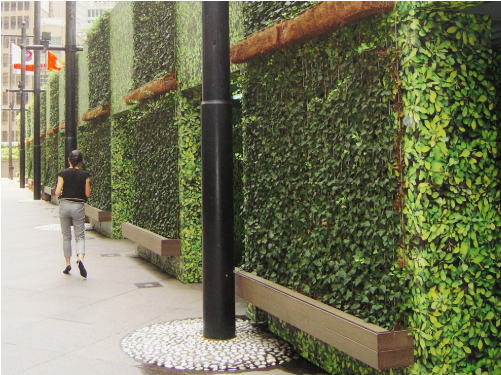
\includegraphics[width=\textwidth]{images/IndirectGreenFacade.png}
		\caption{An Indirect Green Facade \cite{Manso2015}}
		\label{fig:vertical_farm}
	\end{subfigure}
	~
	\begin{subfigure}[b]{0.505\textwidth}
		\centering
		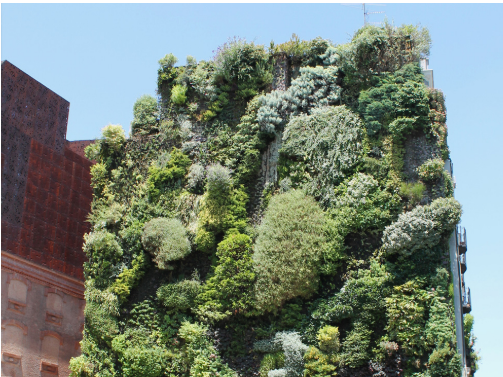
\includegraphics[width=\textwidth]{images/LivingWallSystem}
		\caption{A Living Wall System \cite{Manso2015}}
		\label{fig:vertical_garden}
	\end{subfigure}
	\caption{There exists classifications of vertical wall gardens available in literature \cite{Manso2015}.}
	\label{fig:vertical_applications}
\end{figure}

Of particular interest to the author is the similarity in the applied scenarios of the presented green wall and vertical farming. The two applications can be considered equal in most technical respects, with the main difference largely being the consideration of human consumption qualities in the case of vertical farms. Vertical Farming can be defined as an effort towards the development of sustainable, urban-located agriculture and has attracted considerable industry interest in recent years \cite{Banerjee2014}. Recent market projections indicate a market size estimated to amount to over 2.25 Billion USD by 2024 in the United States alone \cite{Gmi2017}.

The viability of automating vertical wall gardening as well as vertical farming tasks lies in the typically high cost overruns associated with the construction and maintenance of these largely closed ecological systems. This is traditionally done with the help of human labour, with the extenuating risk that these tasks may expose them to (e.g. the scaling of exceedingly tall installations). Additionally, the manual and semi-manual piloting of UAVs can be long and tedious for operators especially when the presence of wind gusts and turbulence is endemic in urban areas; a consequence of the Urban Canyon Effect. The use of a UAV-based, Multi Robot System (UAV-MRS) to achieve the same would drastically reduce this and constitutes a novel approach towards advancing the economic practicality \cite{Bircher2015} of aerial robots in daily human life beyond passing consumer curiosities.

\section{Related Work}

While the determination of standardised metrics to evaluate Swarm and Multi Robot System performance vary from application to application, a number of definitions stand out in the robotics literature that beg mention. In the case of Coverage Path Planning, terms such as path length and time to completion, are present in the literature \cite{Galceran2013} when considering the optimality of generated solutions.

Cuevas et al \cite{Cuevas2013} developed the Social Spider Optimization (SSO) that they comparatively evaluated against the Particle Swarm Optimization (PSO) and Artificial Bee Colony (ABC) algorithms. They utilised a similarly utilised hypothesis testing framework to compare the mean values of each sampled algorithm. In it, they forwarded the Average-Best-So-Far (AB), Median-Best-So-Far (MB) and Standard-Deviation-Best-So-Far (SD) solutions as dependant measurements, testing for a 5\% significance level finding strong evidence against the null hypothesis that assumed no significant difference between the measured sample variables.

Although it is difficult to surface similarly applied research in the literature, there are works that exhibit parallels to this project. Phung et al \cite{Phung2017} developed an enhanced Travelling Salesman Problem (TSP) tractably solved by a discretized PSO algorithm as applied to UAV-based, Structural Health Monitoring (SHM). They formalised Coverage Path Planning (CPP) as a multi-level, Inspection Path Planning (IPP) problem. Their approach alluded to a bipartitioning of the same into an initial Art Gallery Problem, and thereafter optimizing the given solution as a Travelling Salesman Problem. Overlapping photos of the target surfaces are taken once the IPP objective is met for later processing. Guerrero et al \cite{Guerrero2013} similarly presented work on the use of Quadcopters towards the structural inspection of bridges, notably implementing the Path Planning as a Travelling Salesman Problem (TSP). DiFranco et al \cite{DiFranco2015} proposed an energy-aware Coverage Path Planning (CPP) algorithm that minimizes the energy consumption of multi-rotor UAVs while achieving multi-objective surveying of a target space.

Fredslund et al \cite{Fredslund2002} investigated the use of multiple leaders in maintaining formations in Swarm Systems through local sensing and minimal communication i.e. without the sharing of global information with local agents. Matari et al \cite{Matari1995} utilised simple behaviours towards the development of a global flocking behaviour in a group of 13 mobile robots. These behaviours included Safe-Wandering, Following, Dispersion, Aggregation and Homing. A major distinction difference between this project and that of \cite{Matari1995} and \cite{Fredslund2002} is the domain space of the mobile robots. The latter works were implemented on terrestrial-based mobile robots whereas this project considers an application to UAV-based robots. As a matter of observation, the author found there to exist a much larger body of work related to the Swarm and Multi Robot System analysis of terrestrial-based robots. This can be said to be attributable to their rather simpler 2D domain space as compared to UAV-based systems' 3D domain. Bircher et al \cite{Bircher2015} designed and developed a fast algorithm for the efficient inspection path planning of varied structures based and implemented on monolithic UAV systems. They advanced a fast implementation of the Lin-Kernighan-Helsgaun Heuristic (LKH) TSP solver. Optimization of such algorithms is a key area of work in this field due to the limited computing and energy resources available on current aerial quadcopter systems.

\chapter{Implementation} \label{implementation}

In this work, the development of a UAV-MRS towards automated Vertical Wall Gardening is presented in simulation. There exists a wide and diverse problem-set associated with the stated objective that require the interaction of different research domains. This includes but is not limited to UAV stabilization, optimal control, navigation, obstacle avoidance, wireless communications, and computer vision. Measures towards that take resource utilisation and operational cost into account are necessary; It is hoped that the use of an MRS system would help address these issues by employing probabalistic swarm behaviours. Additionally, we forward the usefullness of Swarm Optimization techniques to solving the Coverage Path Planning problem, specifically implementing the Particle Swarm Optimization (PSO) \cite{Kennedy1995} and Ant Colony Optimization (ACO) \cite{Dorigo1997} metaheuristic optimization algorithms.

This work will exclusively make use of this term when referring to the system designed, developed and analysed by the author due to it's applicable semantic definition as a size-constrained robot collective. The considered MRS

 $H_o$ stated thusly, "\textit{Swarm Intelligence and Behaviours do not positively affect task performance in wall-gardening}"

Cao et al's \cite{Cao1988} CPP criteria was adapted through a consideration of a number of limitations:
\begin{itemize}
	\item The utilised SO algorithm implementations are 2D-based and therefore we cannot guarantee that there will be no overlapping paths.
	\item A lack of motion planning features in the ARGoS simulator meant that obstacle avoidance while necessary, would need to be implemented either from the ground up or through planners such as OMPL. Additionally, the lawnmower problem is notable in that it is not designed to account for obstacles \cite{Galceran2013}.
	\item The use of probabilistic behaviours for cooperation control means that complete target area coverage cannot be guaranteed.
\end{itemize}

In this work, a semi-heuristic, offline approach to solving the CPP problem is implemented. In the CPP literature, this is usually solved by cellular decomposition where the target space is broken into sub-regions \cite{Choset2001}. It is formulated as a Travelling Salesman Problem (TSP) and solved with the help of the PSO and ACO Swarm Optimization algorithms. Two key benefits of these algorithms in solving the Travelling Salesman Problem are their relative speed and robustness to combination explosion, an encumbrance to traditional algorithms such as the Cupity Algorithm and the Dynamic Programming Algorithm. However, these benefits come at the cost of optimal global solution guarantees as previously mentioned \cite{Yan2012}.
In this papers' case, the PSO and ACO were selected on account of their prolific prominence in field \cite{Selvi2010}.

In our work, CPP is achieved by two methods:
\begin{itemize}
	\item In the lawn mover motion, a waypoint decomposition of the target space is performed by iteratively generating coordinate points that ascribe to the defined motion. Here, a number of parameters must be set to control the increment steps necessary in the lateral and longitudinal directions.
	\item In the behaviour-based coordination control, a swarm-inspired neighbour-listening approach is used to generate local task waypoint maps for each slave agent. The leader agent is charged with evaluating each plant target as listed in it’s global map.
\end{itemize}

In \cite{Macas2009}, three methods are identified towards the generation and maintainance of shape formations in autonomous, vehicle-based mobile robots:
\begin{itemize}
	\item Virtual Structure.
	\item Behaviour-based.
	\item Leader-following
\end{itemize}
This project proposes a hybrid leader-follower and behaviour-based strategy which is employed to control the navigation of agents in simulation. In the case of the seed-spreader technique, the leader-follower method is the dominant control scheme, with agents strictly concerned with maintaining the virtual hierarchy to ensure optimal inspection coverage.

\section{Experimental Design}
A number of guiding principles \cite{Field2012} were necessarily subscribed to while designing this research experiment:
\begin{itemize}
	\item Empirical.
	\item Measurement.
	\item Replicability.
	\item Objectivity.
\end{itemize}

In aligning to the above, the experimental design was formalized as detailed by Field et al \cite{Field2012} with a research statement developed and posited as follows; "\textit{Do Swarm Intelligence and Behaviours and systems affect the task performance of multi-agent quadcopter systems in wall-gardening}?". The analysis of this affect was undertaken by performing a statistical comparison of naively centralised vs. distributed, metaheuristic-based strategies in task and path planning for multi-agent systems. The posited research question was further refined into the null-hypothesis test, "\textit{Swarm Intelligence and Behaviours do not positively affect task performance in wall-gardening}".

This paper advances an approach towards the implementation, analysis and evaluation of task and path planning in multi-agent systems. In order to infer causality, we must set up two scenarios where the independant variable is present and one where it is absent. These are referred to as the experiment and control conditions with added care taken to ensure they are identical in all senses except for the presence of the cause. This reduces the possibility of \textit{the third variable problem} or \textit{the tertrium quid} where an unidentified, confounding variable effects some unanticipated change in the dependant variable \cite{Field2012}. These latter measures of scenario similarity are covered in \ref{system_design}. In formulating our experiment thusly, the empirical trait requirement of research experiments is met.

Statistical samples for both the control and experiment conditions would need to be generated for analysis, prior to which variable identification must be done. The indepedant/causal variable was characterised as the \textit{usage or non-usage of Swarm Intelligence and Behaviours}. The dependant/outcome variable was selected to be \textit{the simulation-time taken to achieve 90\% task completion coverage}. Given these variable characterisations, the classification of the independant variable can be seen to be a nominal, two-level measure whereas the dependant variable is a parametric, interval measure. Factorial validity of this measure was found to make intuitive sense \cite{Field2012} while it's reliability was ensured by performing multiple trial sampling. Given these prescribed variable types, the student's t test was utilised to compare the means of the two samples \cite{Donald2008}. The parametric characteristic was preferable on account of the following \cite{Field2012}:
\begin{itemize}
	\item There exist a greater variety of tests available that would allow for a wider experimentation base.
	\item Parametric tests are generally better at identifying experimental effects.
\end{itemize}
The generation of sample data qualifies the measurement requirement trait of this experiment.

Replicability was assured by providing a standardized, script-based method of generating new datasets which is elaborated in \ref{system_design}. This is especially pertinent in generating large simulation datasets where parameter setting can be prone to human error. The developed script-based approach provides a single entry point for trial data generation ensuring all necessary parameters are explicitly set, utilised and stored, thereby guarding the mentioned error.

Objectivity.

In the main, a leadership-based, robot organisation strategy was employed which has been shown \cite{Dyer2008} to be an effective method in navigational guidance in the absence. The distinct differences between the control and experimental conditions are listed below:
\begin{itemize}
	\item Navigation path planning.
	\item Local communication.
	\item Global behaviour emergence.
	\item Use of local information.
\end{itemize}

These properties are derived from known swarm robotics characteristics \cite{Dorigo2013}. In navigation path planning, we have centralised and decentralised modes.

The primary method of validation is the comparison between empirical success probabilities and the predicted success probabilities. {Automatic Verification of Autonomous Robot Missions}.

\subsection{Control Condition}
In the control condition, a naive lawn/seed-spreader path planner \cite{Galceran2013} is implemented along with tasked eyebots can travel and probabilistically act on identified targets.
\subsection{Experimental Condition}

\section{System Design} \label{system_design}
The system as presented constitutes a simulation pipeline consisting of the following main subcomponents:
\begin{itemize}
	\item Trial Simulation.
	\item Trial Capture.
	\item Data  Analysis.
\end{itemize}

For this study, trial simulation was performed using the ARGoS simulator, chosen on account of it's ability to simulate large numbers of swarms robots efficiently and flexibly \cite{Pinciroli2014}. This would allow for future work into much larger swarm sizes. In setting up the simulation, the vertical wall-gardening scene environment was purposefully designed to typify a simplified, real-world scenario as shown in Figure \ref{fig:sim_orig_scene}.

\newpage
\begin{figure}
	\begin{subfigure}[b]{0.6\textwidth}
		\centering
		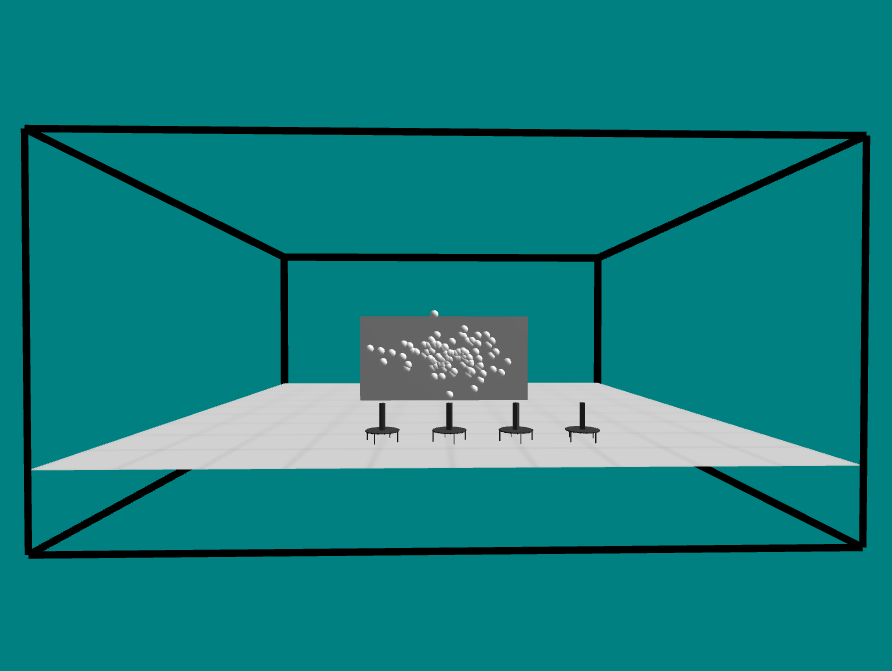
\includegraphics[width=\textwidth]{images/vertical_wall_garden_scene}
		\caption{Simulated Vertical Wall-Gardening Scene}
		\label{fig:sim_orig_scene}
		{The simulated vertical wall-gardening scene run in both control and experiment conditions. The vertical wall is laden with circular (plant) targets with local agents embodied as eye-bot quadcopters}.
	\end{subfigure}
	~
	\begin{subfigure}[b]{0.4\textwidth}
		\centering
		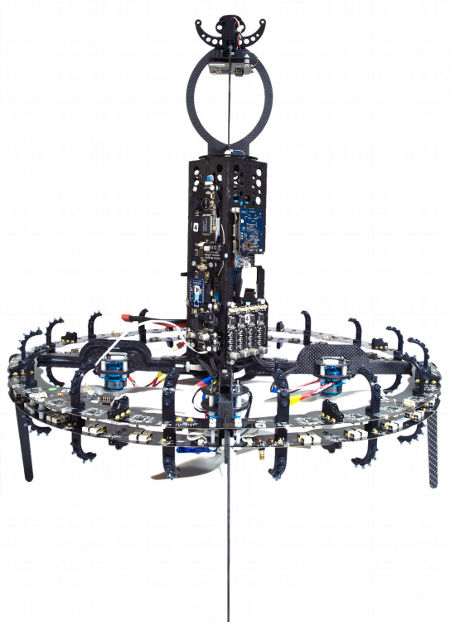
\includegraphics[width=\textwidth]{images/EyebotCarbonFrame}
		\caption{Eyebot Quadcopter}
		\label{fig:eyebot_hardware}
		{Image of a real-world Eyebot, designed and developed as a robotic agent in the Swarminoid Project \cite{Dorigo2013}}.
	\end{subfigure}
	\caption{Simulator Entities}
	\label{fig:sim_orig}
\end{figure}

The swarminoids' \cite{Dorigo2013} eye-bot quadcopter was selected as this studys' simulated, aerial platform due to its' established usage in heterogeneous swarm robotics research. By design, they are autonomous flying robots which can attach to an indoor ceiling, and are capable of analysing the environment from a privileged position to collectively gather information inaccessible to terrestrial-based robots \cite{Dorigo2013}. It is shown in \ref{fig:eyebot_hardware} and features the following sensing capabilities:
\begin{itemize}
    \item Custom $360\deg$ pan-tilt camera system, equipped with a 3MP camera.
    \item Optical $360\deg$ infrared environment distance scanner.
    \item Advanced 3D relative positioning sensor for swarm coordination/communication.
    \item Custom 6-Degree of freedom inertial sensing.
    \item Sonar and differential pressure sensors for altitude determination.
    \item Magnetometer for heading determination.
    \item Horizontal RGB led rings (local visual communication).
\end{itemize}

Additionally, both the control and experimental conditions employ a leader-based multi-agent strategy. PC Capabilities and threading?

\subsection{Uncertainties}
Assuring robot simulation realism is a growing focus area in graphical processing research with notable examples being AirSim \cite{Shah2018} and Morse \cite{Morse2011}.

\subsubsection{Robot and Target Positioning}
Kalman Filtering.
\subsubsection{Target Classification}
\subsubsection{Task and Target Uncertainties}

\subsection{Cooperative Control}

\subsubsection{Task Allocation}
\cite{Bayindir2016} provides a review of swarm robotic tasks and viable techniques used to achieve them.
Swarm robotics systems are characterised by decentralised control, limited communication between robots, use of local information and emergence of global behaviour \cite{Dorigo2013}.To design the organisation systems necessary for robot operation, the task space was delimited to 4 distinct domains:
\begin{itemize}
	\item Evaluation Task.
	\item Water Task.
	\item Nourish Task.
	\item Treatment Task.
\end{itemize}

\subsubsection{Behavioural Design}

\subsection{Path Planning}
One of the critical issues in deploying vehicles in construction sites rests on their navigational abilities [2], particularly, with severe spatial constraints and this naturally leads to the need for formation controls [3]. With this regard, control theoretic [4][5], behaviour-based [6] and A*-based searching [7] approaches have been applied. In the former approach, control designs would be very challenging as precise descriptions or models of the system are required, e.g., in a close-form or differentiable expression, and special consideration may be needed to account for numerical instabilities. On the other hand, the latter approaches require expert design knowledge and behaviours are mostly determined in a problem dependent manner.
Planning Parameters were kept constant for all experiments.

\bgroup
\def\arraystretch{1.5}% 
\begin{table}[h]
  \centering
  \begin{tabular}{|l|c|c|}
  \hline
  \textbf{Planner} & \textbf{Parameter Name} & \textbf{Parameter Value} \\
  \hline
  \multirow{3}{*}{PSO} & Self Trust & 0.2 \\
	& Past Trust & 0.1 \\
	& Global Trust & 0.7 \\
  \hline
  ACO & Number of Ants & 10 \\
  \hline
  \multirow{3}{*}{LAWN} & Launch Step & 500 \\
	& Horizontal Step & 0.1 \\
	& Vertical Step & 0.1 \\
  \hline
  \end{tabular}
  \caption{This table shows some data}
  \label{tab:myfirsttable}
\end{table}
\egroup

\subsubsection{Particle Swarm Optimization}
\subsubsection{Ant Colony Optimization}
\subsubsection{Lawn Sweeping Strategy}
Cao et al \cite{Cao1988} introduced a region filling strategy for sweeping operations in a robot lawn mower (RLM), thereby setting the stage for advanced studies into coverage path planning (CPP) strategies \cite{Galceran2013}. In this work, we implement the a similar region filling strategy, with one caveat being the lack of obstacle avoidance and replanning.

\section{Data Collection}

\chapter{Evaluation} \label{evaluation}

\begin{figure}[h]
	\begin{subfigure}[b]{0.5\textwidth}
		\centering
		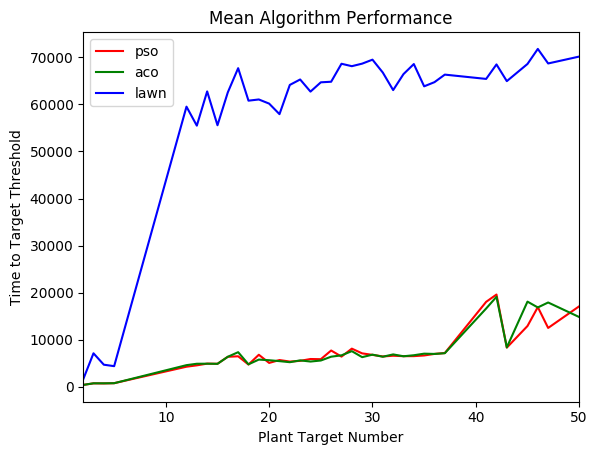
\includegraphics[width=\textwidth]{images/all_means_line_plot}
		\caption{Means Line Plot}
		\label{fig:means_line}
	\end{subfigure}
	~
	\begin{subfigure}[b]{0.5\textwidth}
		\centering
		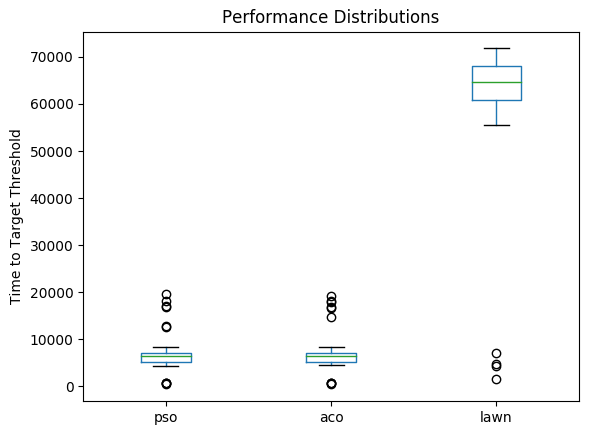
\includegraphics[width=\textwidth]{images/all_means_box_plot}
		\caption{Means Box Plot}
		\label{fig:means_box}
	\end{subfigure}
	\caption{Algorithm Performances}
	\label{fig:means_stat}
\end{figure}

\chapter{Conclusion} \label{conclusion}
Future work into leaderless, self-organisation strategies with greater swarm sizes. The former can be achieved via agent roaming procedures that incorporate random walk behaviour with swarm cohesion implemented through Leinard-Jones potentials between agents.
Contributions include a programmatic framework for the generation of simulation data suitable for biological statistical analysis. The need for benchmark datasets in the field is a noted need and it is hoped that added effort is placed towards the release of standardised benchmarking sets.
Established path planners such as Open Motion Planning Library (OMPL) \cite{Sucan2012} should be considered for enhanced validity in comperative analyses. Further, higher order models of the quadcopter and external disturbances such as wind should be considered to enhance simulator realism. Higher order models are possible employing techniques to generating models learned from flight data \cite{Symington2014} whereas robust wind models such as the Dryden wind turbulence model \cite{Dryden} could be included. Collision detection and obstacle avaoidance with 3D-capable metaheuristic planners. Techniques and approaches to parameter optimisation and social learning such as genetic programming or neural networks are high potential, interest areas that would be considered to augment this work in future.
A standardised metaheuristic optimization algorithm library such as \cite{James2018} and a wider variety state prediction techniques such as probabilistic smoothing.
SLAM Mapping of targets.
Multi-objective TSP.
Enhanced local communication with the ring leds.
Implement time estimation techniques to vary holding times.
A dataset repository of similarly generated simulation data.
There is still much to be desired in the terminology and frameworks available in literature.
As explained in the introduction of \cite{Phung2017}, Implement the DPSO in a GPU-based framework so that the computation time can be significantly reduced while keeping the hardware requirement unchanged.
A better integrated simulator such as MORSE that utilises Blender as its' 3D modelling engine would allow for more visually realistic scenes. Alternatively, AirSim, a recently released autonomous vehicle simulation platform could be used. This would open the field to novel behaviour modelling approaches via deep learning, a field in recent resurgence due to enhanced GPU computing capabilities and access to swaths of training data.
Studies in to the response of the MRS to adaptivity and fault tolerance (Iocchi2001).

\appendix
\bibliographystyle{plain}
\bibliography{references/Library,references/Misc}
\chapter{Code listing}

\end{document}